%; whizzy paragraph -pdf xpdf -latex ./whizzypdfptex.sh
%; whizzy-paragraph "^\\\\begin{frame}\\|\\\\emtext"
% latex beamer presentation.
% platex, latex-beamer でコンパイルすることを想定。 

%     Tokyo Debian Meeting resources
%     Copyright (C) 2012 Junichi Uekawa

%     This program is free software; you can redistribute it and/or modify
%     it under the terms of the GNU General Public License as published by
%     the Free Software Foundation; either version 2 of the License, or
%     (at your option) any later version.

%     This program is distributed in the hope that it will be useful,
%     but WITHOUT ANY WARRANTY; without even the implied warreanty of
%     MERCHANTABILITY or FITNESS FOR A PARTICULAR PURPOSE.  See the
%     GNU General Public License for more details.

%     You should have received a copy of the GNU General Public License
%     along with this program; if not, write to the Free Software
%     Foundation, Inc., 51 Franklin St, Fifth Floor, Boston, MA  02110-1301 USA

\documentclass[cjk,dvipdfmx,12pt]{beamer}
\usetheme{Tokyo}
\usepackage{monthlypresentation}

%  preview (shell-command (concat "evince " (replace-regexp-in-string "tex$" "pdf"(buffer-file-name)) "&")) 
%  presentation (shell-command (concat "xpdf -fullscreen " (replace-regexp-in-string "tex$" "pdf"(buffer-file-name)) "&"))
%  presentation (shell-command (concat "evince " (replace-regexp-in-string "tex$" "pdf"(buffer-file-name)) "&"))

%http://www.naney.org/diki/dk/hyperref.html
%日本語EUC系環境の時
\AtBeginDvi{\special{pdf:tounicode EUC-UCS2}}
%シフトJIS系環境の時
%\AtBeginDvi{\special{pdf:tounicode 90ms-RKSJ-UCS2}}

\newenvironment{commandlinesmall}%
{\VerbatimEnvironment
  \begin{Sbox}\begin{minipage}{1.0\hsize}\begin{fontsize}{8}{8} \begin{BVerbatim}}%
{\end{BVerbatim}\end{fontsize}\end{minipage}\end{Sbox}
  \setlength{\fboxsep}{8pt}
% start on a new paragraph

\vspace{6pt}% skip before
\fcolorbox{dancerdarkblue}{dancerlightblue}{\TheSbox}

\vspace{6pt}% skip after
}
%end of commandlinesmall


\title{Raspberry Pi 2 Model B に Debian Jessie / armhf をインストールする}
\subtitle{第125回 2015年3月度}
\author{岩松 信洋}
\date{2015年3月7日}
\logo{
\includegraphics[width=8cm]{image200607/openlogo-light.eps}}

\begin{document}

\begin{frame}
\titlepage{}
\end{frame}

\begin{frame}{アジェンダ}
\begin{enumerate}
\item Raspberry Pi 2 Model B と Raspberry Pi の違い
\item Raspberry Pi 2 Model B に Debian Jessie / armhf をインストールする
\end{enumerate}
\end{frame}



\emtext{Raspberry Pi 2 Model B と Raspberry Pi の違い}

\begin{frame}{Raspberry Pi 2とは?}
\begin{itemize}
\item 2015年2月2日に発売された新しい Raspberry Pi
\item CPU、メモリの強化
\item Raspberry Pi 2 では Debian armhf が利用できる
\item Raspbian 使わなくても良くなった。
\item Raspbian is not Debian
\end{itemize}
\end{frame}

\begin{frame}{Raspberry Pi 2 Model B と Raspberry Pi の違い}
\begin{figure}[htbp]
\begin{center}
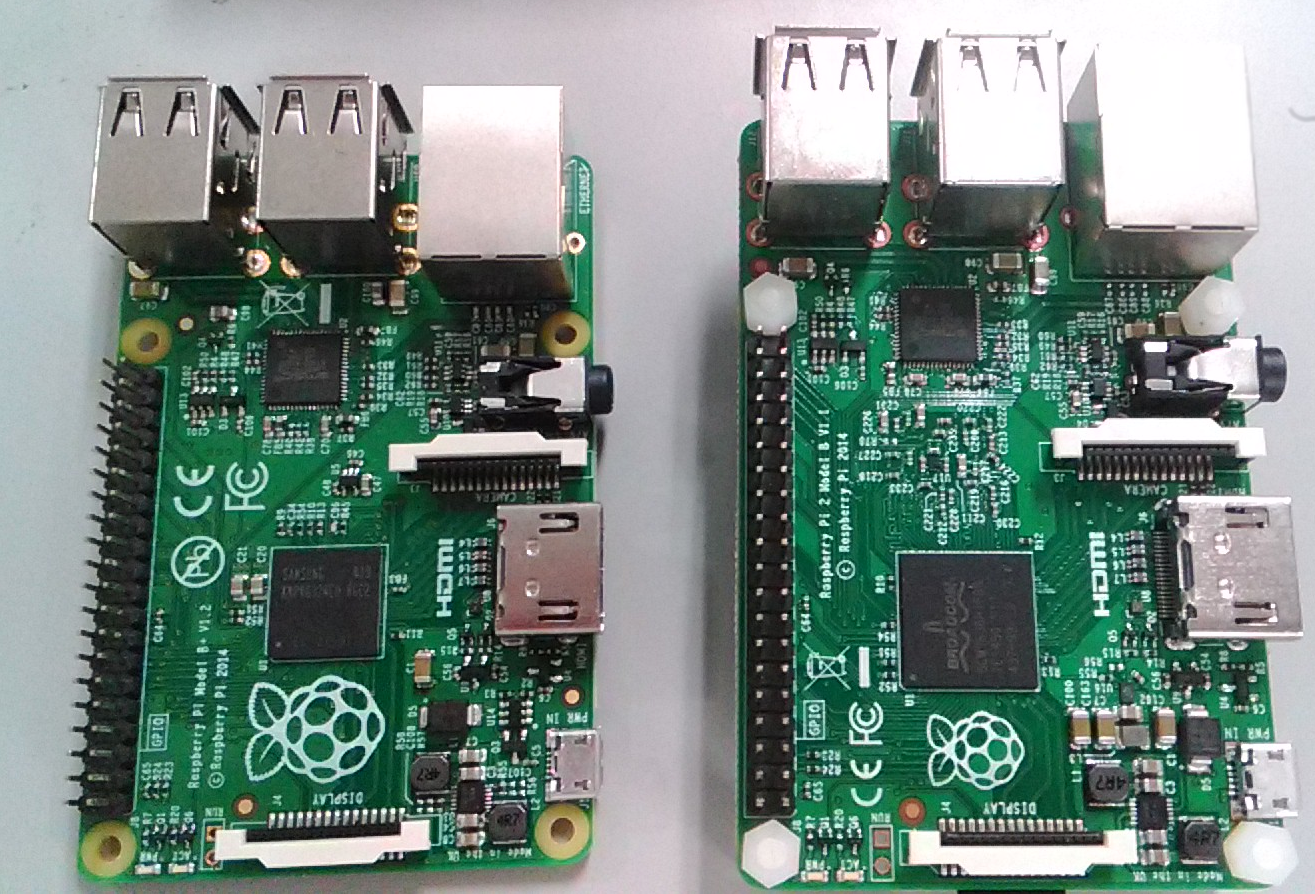
\includegraphics[width=0.7\hsize]{image201503/rpis.png}
\end{center}
\end{figure}
\end{frame}

\begin{frame}[containsverbatim]{Raspberry Pi 2 Model B と Raspberry Pi の違い}

\resizebox{\textwidth}{!}{
\begin{tabular}{|c|c|c|}
\hline
-   & RPi Model B+ & RPi 2 Model B \\
\hline
\hline
CPU  & ARM1176JZF-S 1コア (700MHz) / ARMv6 & {\color{red}ARM Cortex-A7 4コア (900MHz) / ARMv7}\\
\hline
SoC  & Broadcom BCM2835 &  Broadcom BCM2836 \\  
\hline
CPU  & Broadcom VideoCore IV (250MHz) & 同左 \\
\hline
メモリ & 512MB (SDRAM)& {\color{red}1GB (LPDDR2 SDRAM)} \\
\hline
ネットワーク & LAN9514 (10/100 Mbps) & 同左 \\
\hline
外部I/O & GPIO 40ピン & 同左 \\
\hline
ストレージ & microSD & 同左 \\
\hline
電源 & 600 mA (3.0W) & {\color{red}900 mA (4.5-5.5W)} \\
\hline
\end{tabular}
}
\end{frame}

\begin{frame}{Raspberry Pi 2 Model B と Raspberry Pi の違い}

\resizebox{\textwidth}{!}{
\begin{tabular}{|c|c|c|c|}
\hline
 - & Debian armel & Debian armhf & Raspbian \\
\hline
\hline
ターゲット命令セット &  ARMv4 & ARMv7 & ARMv6 \\
\hline
FPU &  なし &  VFPv3  &  VFPv2 \\
\hline
Debian ネイティブ & Yes & Yes & No \\
\hline
\end{tabular}
}
\end{frame}

\begin{frame}{Raspberry Pi 2 Model B と Raspberry Pi の違い}

Unixbench (System Benchmarks Index Score) 
\resizebox{\textwidth}{!}{
\begin{tabular}{|c|c|c|c|}
\hline
Debian armel / RPi & Debian armhf /RPi2 & Raspbian / Rpi & Raspbian / Rpi2 \\
\hline
66.5 & 450.8 (183.1) & 80.1 & 442.9 (173.8) \\
\hline
\end{tabular}
}
\end{frame}

\emtext{Debian armhf / Jessie のインストール方法}

\begin{frame}{Debian armhf / Jessie のインストール方法}

準備するもの

\begin{itemize}
\item 実機
\item 初期化されてもよい4GB以上のmicroSDカード
\item 電源用のmicro USB ケーブル
\item USBシリアル変換モジュール
\end{itemize}

\end{frame}

\begin{frame}{接続例}
\begin{figure}[htbp]
\begin{center}
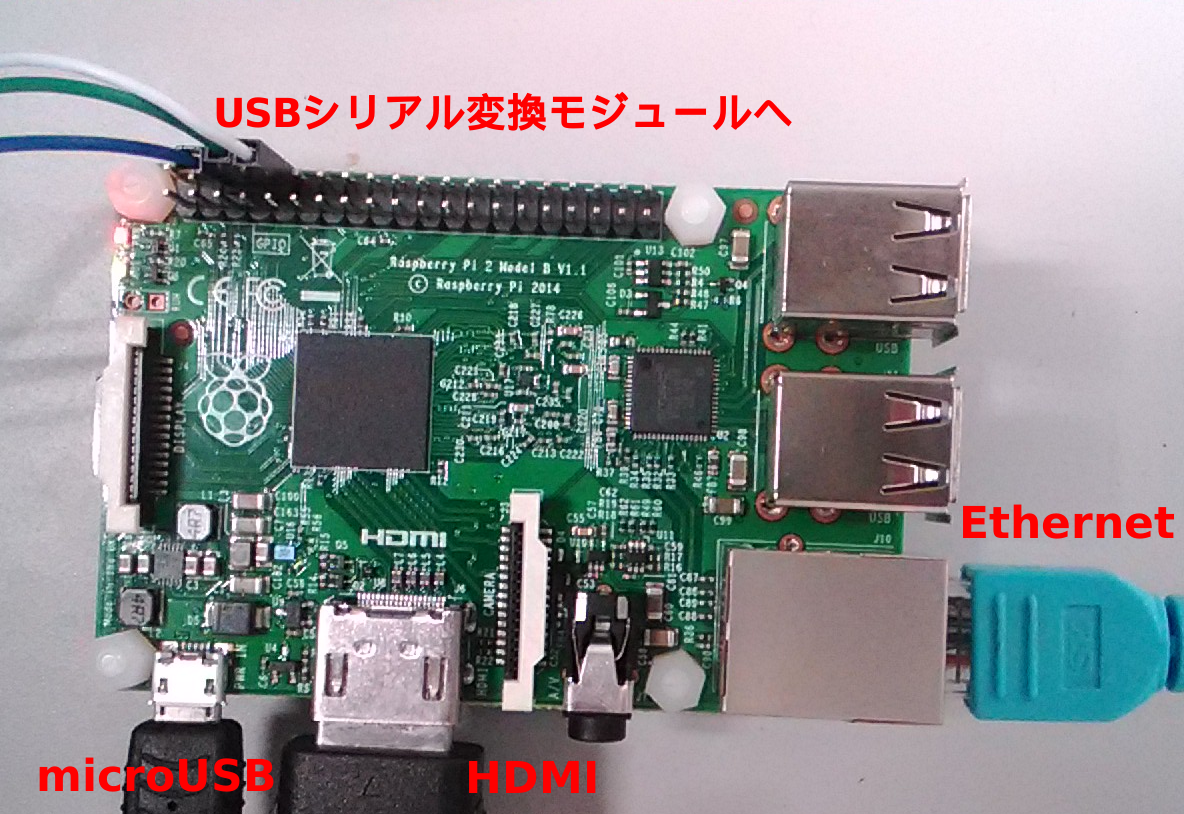
\includegraphics[width=0.7\hsize]{image201503/rpi2-hw-setting.png}
\end{center}
\caption{RPi2 接続例}
\label{fig:rpi2-hw-setting}
\end{figure}
\end{frame}

\begin{frame}{作業の流れ}
\begin{enumerate}
\item microSDカードの認識確認
\item microSDカードの初期化
\item microSDカードにパーティション作成
\item microSDカードのフォーマット
\item cdebootstrap を使ってmicroSDカードにインストール
\item RPi2のLinuxカーネルとカーネルモジュールのインストール
\item RPi2のカーネルコマンドラインの設定
\item fstabの設定
\item ネットワークデバイスの設定
\item rootfs用パーティションの変更
\item root のパスワードの設定とrpiユーザの追加
\item microSDカードのアンマウントとRPi2の起動
\item RPi2 へのログイン
\item RPi2 専用ツールのインストール
\end{enumerate}
\end{frame}

\begin{frame}{non native cdebootstrap}
\begin{center}
\includegraphics[width=0.7\hsize]{image201503/cdebootstrap.eps}
\end{center}
\end{frame}

\begin{frame}[containsverbatim]{microSDカードの認識確認}

\begin{commandline}
$ dmesg  | tail -5
[858983.896718] FAT-fs (sdf1): Directory bread(block 32775) failed
[858983.896729] FAT-fs (sdf1): Directory bread(block 1390704) failed
[858983.896731] FAT-fs (sdf1): Directory bread(block 1390705) failed
[869873.800361] sd 6:0:0:3: [sde] 15523840 512-byte logical blocks: (7.94 GB/7.40 GiB)
[869873.831121]  sde: sde1
\end{commandline}

\end{frame}

\begin{frame}[containsverbatim]{microSDカードの初期化}

\begin{commandline}
$ sudo dd if=/dev/zero of=/dev/sde bs=1M count=1
\end{commandline}

\end{frame}

\begin{frame}[containsverbatim]{microSDカードにパーティション作成}

\begin{commandline}
$ sudo fdisk /dev/sde
Command (m for help): o
...
Command (m for help): n
...
Select (default p): p
...
Partition number (1-4, default 1): 1
...
Last sector, +sectors or +size{K,M,G,T,P} \
	     (2048-15523839, default 15523839): +32M
...
Command (m for help): t
...
Hex code (type L to list all codes): e
...
Command (m for help): n
...
Select (default p): p
...
Partition number (2-4, default 2): 2
...
Command (m for help): w
\end{commandline}

\end{frame}

\begin{frame}[containsverbatim]
\begin{commandline}
(echo o; echo n; echo p; echo 1; echo ; echo +32M; \
 echo t; echo e; echo n; echo p; echo 2; echo ; echo ; \
 echo w) | fdisk /dev/sde
\end{commandline}
\end{frame}

\begin{frame}[containsverbatim]{microSDカードのフォーマット}

\begin{commandline}
$ sudo mkfs.msdos /dev/sde1
$ sudo mkfs.ext4 /dev/sde2
$ mkdir /tmp/boot /tmp/rootfs
$ sudo mount /dev/sde1 /tmp/boot
$ sudo mount /dev/sde2 /tmp/rootfs
\end{commandline}
\end{frame}

\begin{frame}[containsverbatim]{cdebootstrap を使ってmicroSDカードにインストール}

\begin{commandline}
$ sudo cdebootstrap --arch=armhf -f standard \
  --foreign jessie \
  --include=openssh-server,ntp,ca-certificates,vim \
  /tmp/rootfs
...
\end{commandline}

\end{frame}

\begin{frame}[containsverbatim]{RPi2のLinuxカーネルとカーネルモジュールのインストール}

\begin{itemize}
\item RPi2のLinuxカーネルはDebianでは提供されていない
\item 完全にアップストリームでサポートされていない
\item 起動にファームウェアが必要
\item Debianで RPi2 のLinuxカーネルを扱うにはrpi-update を使って最新カーネルをコピーする
\end{itemize}

\end{frame}

\begin{frame}[containsverbatim]{RPi2のLinuxカーネルとカーネルモジュールのインストール}
\begin{commandline}
$ sudo curl -o /tmp/rootfs/usr/bin/rpi-update https://raw.githubusercontent.com/Hexxeh/rpi-update/master/rpi-update
$ sudo chmod +x /tmp/rootfs/usr/bin/rpi-update
$ sudo mkdir /tmp/rootfs/lib/modules
$ sudo ROOT_PATH=/tmp/rootfs BOOT_PATH=/tmp/boot /tmp/rootfs/usr/bin/rpi-update
*** Raspberry Pi firmware updater by Hexxeh, enhanced by AndrewS and Dom 
 *** Performing self-update
  % Total    % Received % Xferd  Average Speed   Time    Time     Time  Current
                                 Dload  Upload   Total   Spent    Left  Speed
100  8107  100  8107    0     0  54471      0 --:--:-- --:--:-- --:--:-- 54777
 *** Relaunching after update
...
\end{commandline}
\end{frame}

\begin{frame}[containsverbatim]{RPi2のカーネルコマンドラインの設定}

\begin{commandline}
$ sudo sh -c "echo dwc_otg.lpm_enable=0 console=ttyAMA0,115200 console=tty1
     root=/dev/mmcblk0p2 rootwait > /tmp/boot/cmdline.txt
\end{commandline}
\end{frame}

\begin{frame}[containsverbatim]{fstabの設定}

\begin{commandline}
proc            /proc           proc    defaults	0	0
/dev/mmcblk0p1  /boot           vfat    defaults	0	2
/dev/mmcblk0p2  /               ext4    defaults,noatime	0	1
\end{commandline}

\end{frame}

\begin{frame}[containsverbatim]{ネットワークデバイスの設定}

\begin{commandline}
auto eth0
iface eth0 inet dhcp
\end{commandline}
\end{frame}

\begin{frame}[containsverbatim]{rootfs用パーティションの変更}

\begin{commandline}
trap 'error "Interruped!"' HUP INT TERM

mount -n -o remount,rw rootfs / <- これを
mount -n -o remount,rw /dev/mmcblk0p2 / <- これに変更

chown -hR 0:0 /
\end{commandline}
\end{frame}

\begin{frame}[containsverbatim]{root のパスワードの設定とrpiユーザの追加}
\begin{commandline}
echo 'deb http://ftp.debian.org/debian jessie main' > /etc/apt/sources.list

echo "root:root" | chpasswd <- この行を追加
useradd -m rpi <- この行を追加
echo rpi:rpi | chpasswd <- この行を追加

run rm /sbin/init
\end{commandline}
\end{frame}

\begin{frame}[containsverbatim]{microSDカードのアンマウントとRPi2の起動}

\begin{enumerate}
\item microSDカードをアンマウントし、PRi2 の microSDカードスロットに挿入する。
\item 挿入後、micro USB ケーブルを RPi2 に挿し、RPi2を起動する。
\item 起動すると自動的に2nd bootstrapが実行され、RPi2上でインストールが実行される
\item 30分ほど待つ
\item インストール完了
\end{enumerate}
\end{frame}

\begin{frame}[containsverbatim]{RPi2 へのログイン}

\begin{itemize}
\item USBシリアルモジュール経由
\item SSH 経由
\item HDMI モニタ(tty)経由
\end{itemize}

\end{frame}

\begin{frame}[containsverbatim]{RPi2 専用ツールのインストール}

\begin{itemize}
\item RPi の専用ツールである rpi-update、raspi-config はまだDebian
では提供されていない
\item これらを Debian で利用できるようにするには raspberrypi.org で提供されている 各ツールの
Debian パッケージをインストールする必要がある。
\end{itemize}

\end{frame}

\begin{frame}[containsverbatim]{RPi2 専用ツールのインストール}

\begin{commandline}
# wget -O - http://archive.raspberrypi.org/debian/raspberrypi.gpg.key | apt-key add - 
# echo deb http://archive.raspberrypi.org/debian wheezy main >> /etc/apt/sources.list
# apt-get update
# apt-get install rpi-update raspi-config
\end{commandline}
\end{frame}

\begin{frame}{終わりに}

\begin{itemize}
\item RPi2 から ネイティブのDebianが利用できるようになった
\item インストーラやmicroSDカードイメージが準備されていなくても、cdebootstrap 
使えば簡単にインストールできる
\item Raspbian is not Debian。RPi2 ではDebianを使いましょう。
\end{itemize}

\end{frame}

\end{document}

;;; Local Variables: ***
;;; outline-regexp: "\\([ 	]*\\\\\\(documentstyle\\|documentclass\\|emtext\\|section\\|begin{frame}\\)\\*?[ 	]*[[{]\\|[]+\\)" ***
;;; End: ***
